\documentclass[12pt, a4paper]{article}
\usepackage[utf8]{inputenc}
\usepackage{listings}
\usepackage[IL2]{fontenc}
\usepackage[czech]{babel}
\usepackage{graphicx}
\usepackage{mathtools}
\usepackage{amsmath}
\usepackage[pdfborder={0 0 0}]{hyperref}

\title{\textbf{Dokumentace semestrální práce} \\KIV/PT}
\author{Vojtěch Danišík}
\begin{document}

\begin{titlepage} 
	\newcommand{\HRule}{\rule{\linewidth}{0.5mm}} 
	\begin{center}
	
\includegraphics[width=6cm]{img/logo}\\
	\end{center}
	\textsc{\LARGE Západočeská univerzita v~Plzni}\\[1.5cm] 	
	\textsc{\Large Mobilní komunikace a zařízení}\\[0.5cm] 
	\textsc{\large KIV/MKZ}\\[0.5cm] 
	\HRule\\[0.4cm]
	{\huge\bfseries Dokumentace semestrální práce}\\[0.4cm] 
	\HRule\\[1.5cm]

	\begin{minipage}{0.4\textwidth}
		\begin{flushleft}
			\large
			Vojtěch \textsc{Danišík}\newline
			A16B0019P\newline
			danisik@students.zcu.cz
		\end{flushleft}
	\end{minipage}
	\vfill\vfill\vfill
	\begin{flushright}
	{\large\today}
	\end{flushright}
	\vfill 
\end{titlepage}
\newpage
\tableofcontents
\newpage
\section{Zadání}
Jako zadání semestrální práce pro předmět MKZ byla vybrána hra \textbf{Hledání min - Minesweeper}. Hlavní podstatou hledání min je do stanoveného času označkovat pomocí vlajek políčka, která nebyla ještě odhalena a pod kterými se mohou nacházet bomby. Pokud hráč klikne na políčko, která obsahovala bombu, tak bomba vybuchne a hra končí neúspěchem. Počet vlajek ve hře je roven počtu bomb rozmístěných náhodně po celé hrací ploše. Pokud hráč klikne na políčko, které nesousedí ani s~jednou bombou, je pole odkryto do té doby, dokud všechna nově objevená políčka nemají ve svém okolí alespoň jednu bombu. Čísla, která se ukáží po kliknutí na políčko značí počet bomb sousedících s~aktuálně kliknutým políčkem. Vzhled této hry lze vidět na obrázku \ref{fig:uvod_obrazek}.
	\begin{figure}[h!]
	\centering
	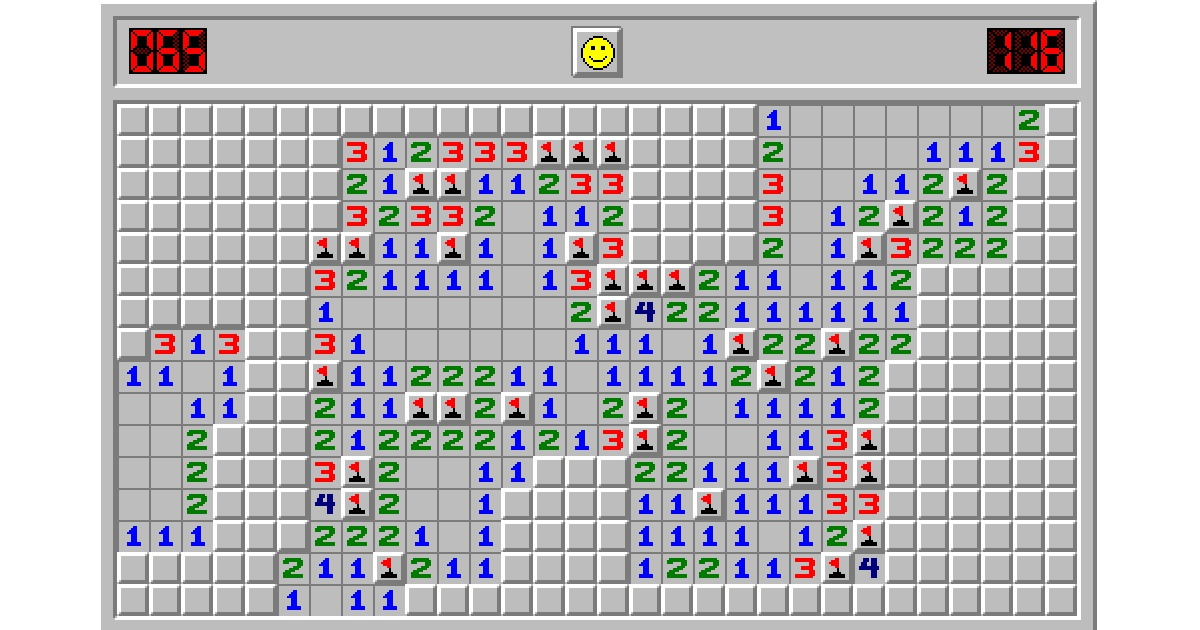
\includegraphics[width=14cm]{img/uvod_obrazek}\\
	\caption{Hledání min - ukázka}
	\label{fig:uvod_obrazek}
	\end{figure}
\newpage


\section{Programátorská dokumentace}
V~programu bylo použito pro docílení správné funkcionality 7 tříd, z~toho jedna abstraktní.
\par
Třída \textbf{MainActivity} slouží jako hlavní třída aplikace. V~této třídě se děje zobrazování již vytvořených struktur, jako jsou například časovač, hrací panel ale také i přiřazování aktivit pro tlačítka RESET a SET FLAG.
\par
Třída \textbf{GameEngine} obsahuje funkční kód hrací plochy a tlačítek samotných. Při kliknutí na jednotlivé tlačítko je zavolána metoda \textit{click}, která má za úkol zjistit mód ve kterém se uživatel nachází (zda odhaluje bomby nebo dává vlajky) a následně podle toho udělat určitou aktivitu. Zároveň se po každém kliknutí kontroluje, zda není hra dohrána pomocí metody \textit{checkEnd}, ale i zda uživatel nezvolil tlačítko, které obsahuje bombu.
\par
Třída \textbf{Generator} má za úkol vytvořit celou hrací plochu a všech tlačítek. Nejdříve jsou vytvořena políčka bez jakéhokoliv označení, pouze jsou náhodně vygenerovány pozice políček, na kterých bude vložena bomba. Po vygenerování všech políček probíhá vypočítání čísla políčka, které značí počet bomb, které se vyskytují v~blízkosti aktuálně zpracovávaného políčka viz obrázek \ref{fig:sousedi}.
	\begin{figure}[h!]
	\centering
	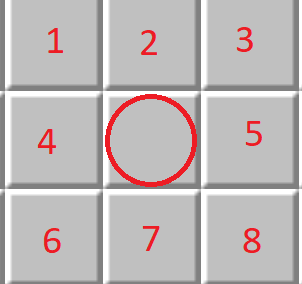
\includegraphics[width=5cm]{img/sousedi}\\
	\caption{Sousední políčka, která mohou potencionálně obsahovat bombu}
	\label{fig:sousedi}
	\end{figure}
\par
Abstraktní třída \textbf{BaseCell} má za úkol připravit strukturu pro políčko, které bude vloženo do hracího pole. Obsahuje proměnné udávají zda je políčko bomba, jestli je označené vlajkou, zda je odhaledno a hodnotu udávající počet sousedních bomb doplněno o~pozici v~hracím poli.
\par
Třída \textbf{Cell} rozšiřuje námi vytvořenou abstraktní třídu BaseCell. Hlavním úkolem této třídy je přiřadit na základě stanovených hodnot (ve třídě BaseCell), jaký obrázek bude použit při vykreslení (při neodhalení, po odhalení zda se jedná o~bombu nebo pouze obsahuje číslo udávající počet sousedních bomb).
\par
Třída \textbf{Grid} zařizuje vytvoření veškerých struktur, které jsou dále poslány třídě MainActivity. Pro splnění tohoto účelu byla vytvořena private třída \textbf{GridAdapter}, která slouží jako most mezi námi vytvořenými daty a jejich vyobrazením.
\newpage


\section{Uživatelská dokumentace}
\subsection{Vzhled aplikace}
Výsledný vzhled aplikace lze vidět na několika obrázcích. První obrázek (viz \ref{fig:uvodni}) vyobrazuje aplikaci po jejím spuštění. Trochu se liší od původního vzhledu aplikace (viz \ref{fig:uvod_obrazek}), časovač a čítač vlajek je posunut pod hrací pole.
	\begin{figure}[h!]
	\centering
	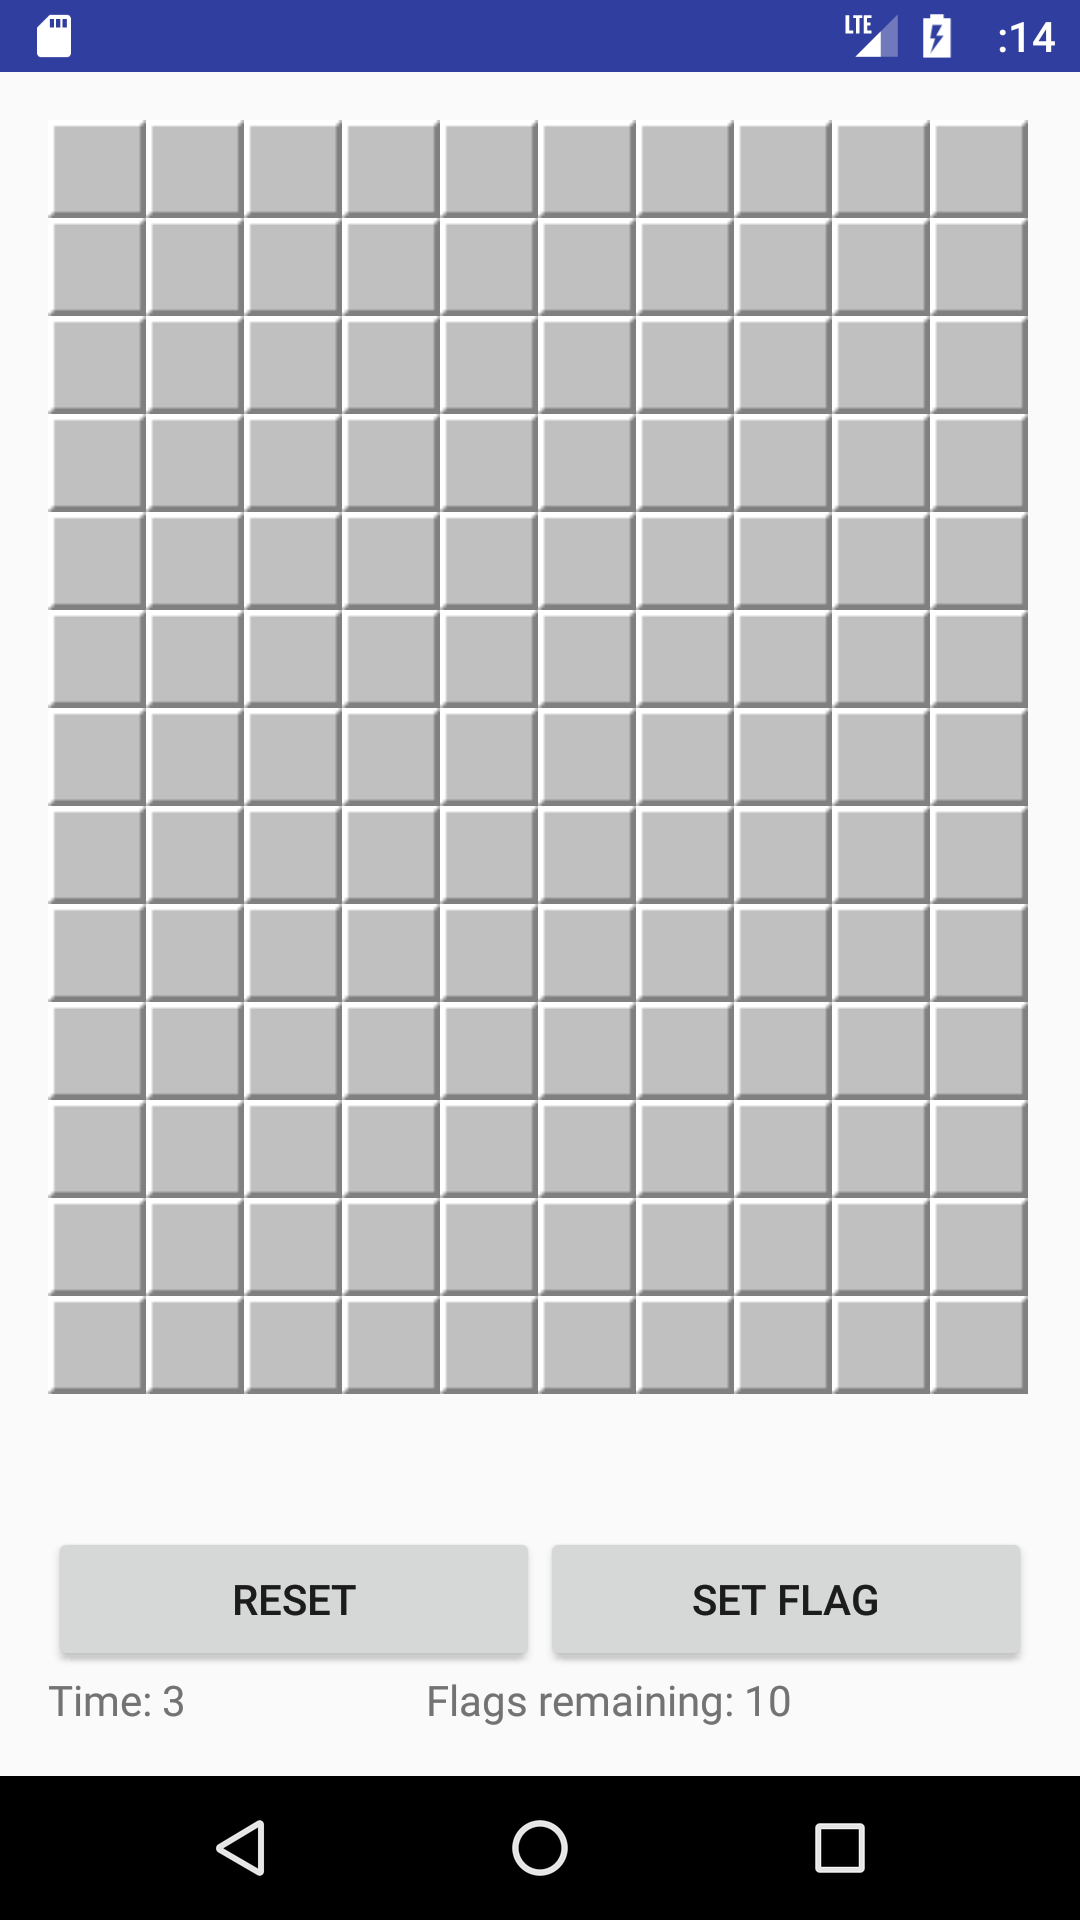
\includegraphics[width=4cm]{img/uvodni}\\
	\caption{Vzhled aplikace}
	\label{fig:uvodni}
	\end{figure}
\par
Do aplikace byly následně přidány i dvě tlačítka. Levé tlačítko \textit{RESET} má za úkol vrátit již rozehranou hru do původního stavu (ať už uprostřed hry nebo po prohře). Druhé tlačítko \textit{SET FLAG/DISABLE FLAG} má za úkol měnit stav hraní při kliknutí. Po prvním stisknutí je zapnut stav pokládání vlajek, zatímco po druhém je stav vrácen do původního a hráč může dále objevovat stále neobjevená políčka. Příklad vlajek lze vidět na obrázku \ref{fig:vlajky}.
\newpage
	\begin{figure}[h!]
	\centering
	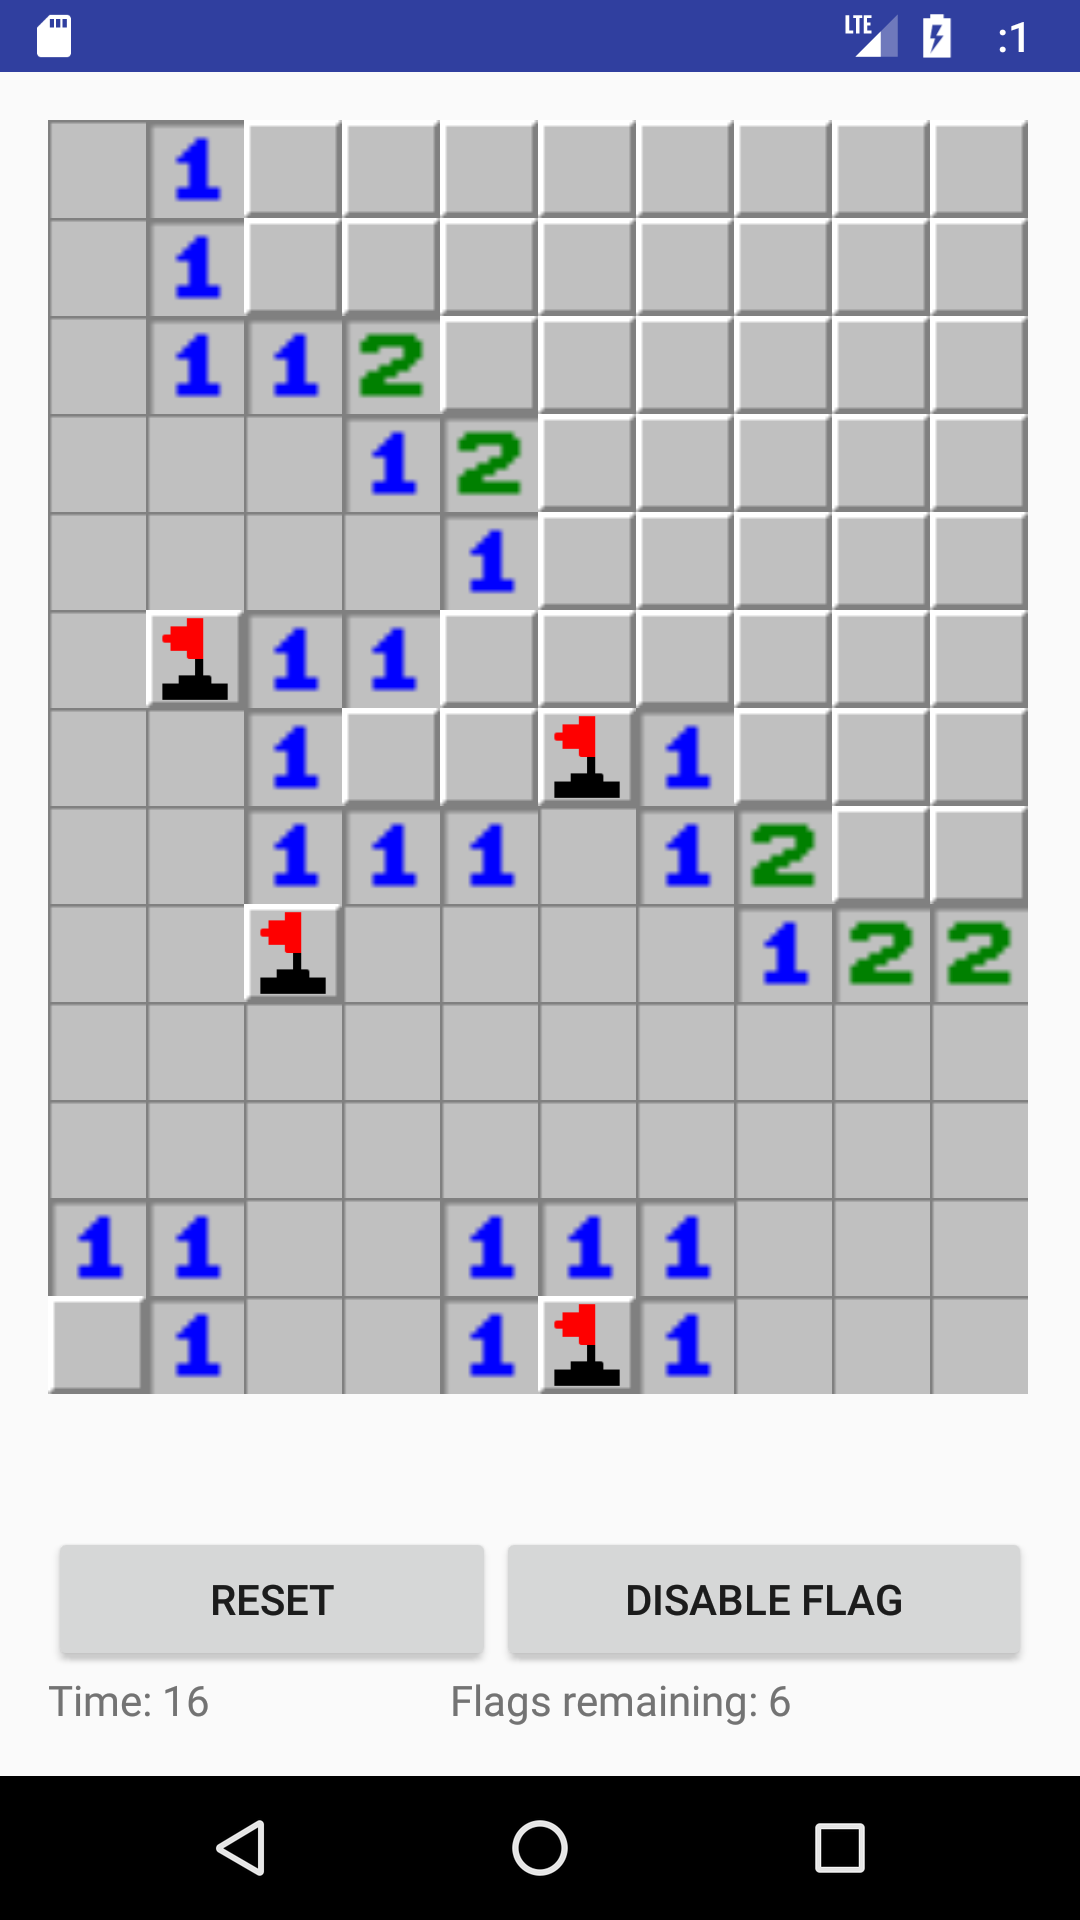
\includegraphics[width=4cm]{img/vlajky}\\
	\caption{Využití vlajek pro označení bomb}
	\label{fig:vlajky}
	\end{figure}
\par
Pokud uživatel při odhalování hracího pole narazí na bombu, pak je tato bomba zvýrazněna, ostatní bomby jsou odhaleny a hra končí. Následně má uživatel možnost hru opakovat stisknutím tlačítka \textit{RESET} nebo hru ukončit. Příklad kliknutí na bombu lze vidět na obrázku \ref{fig:prohra}.
	\begin{figure}[h!]
	\centering
	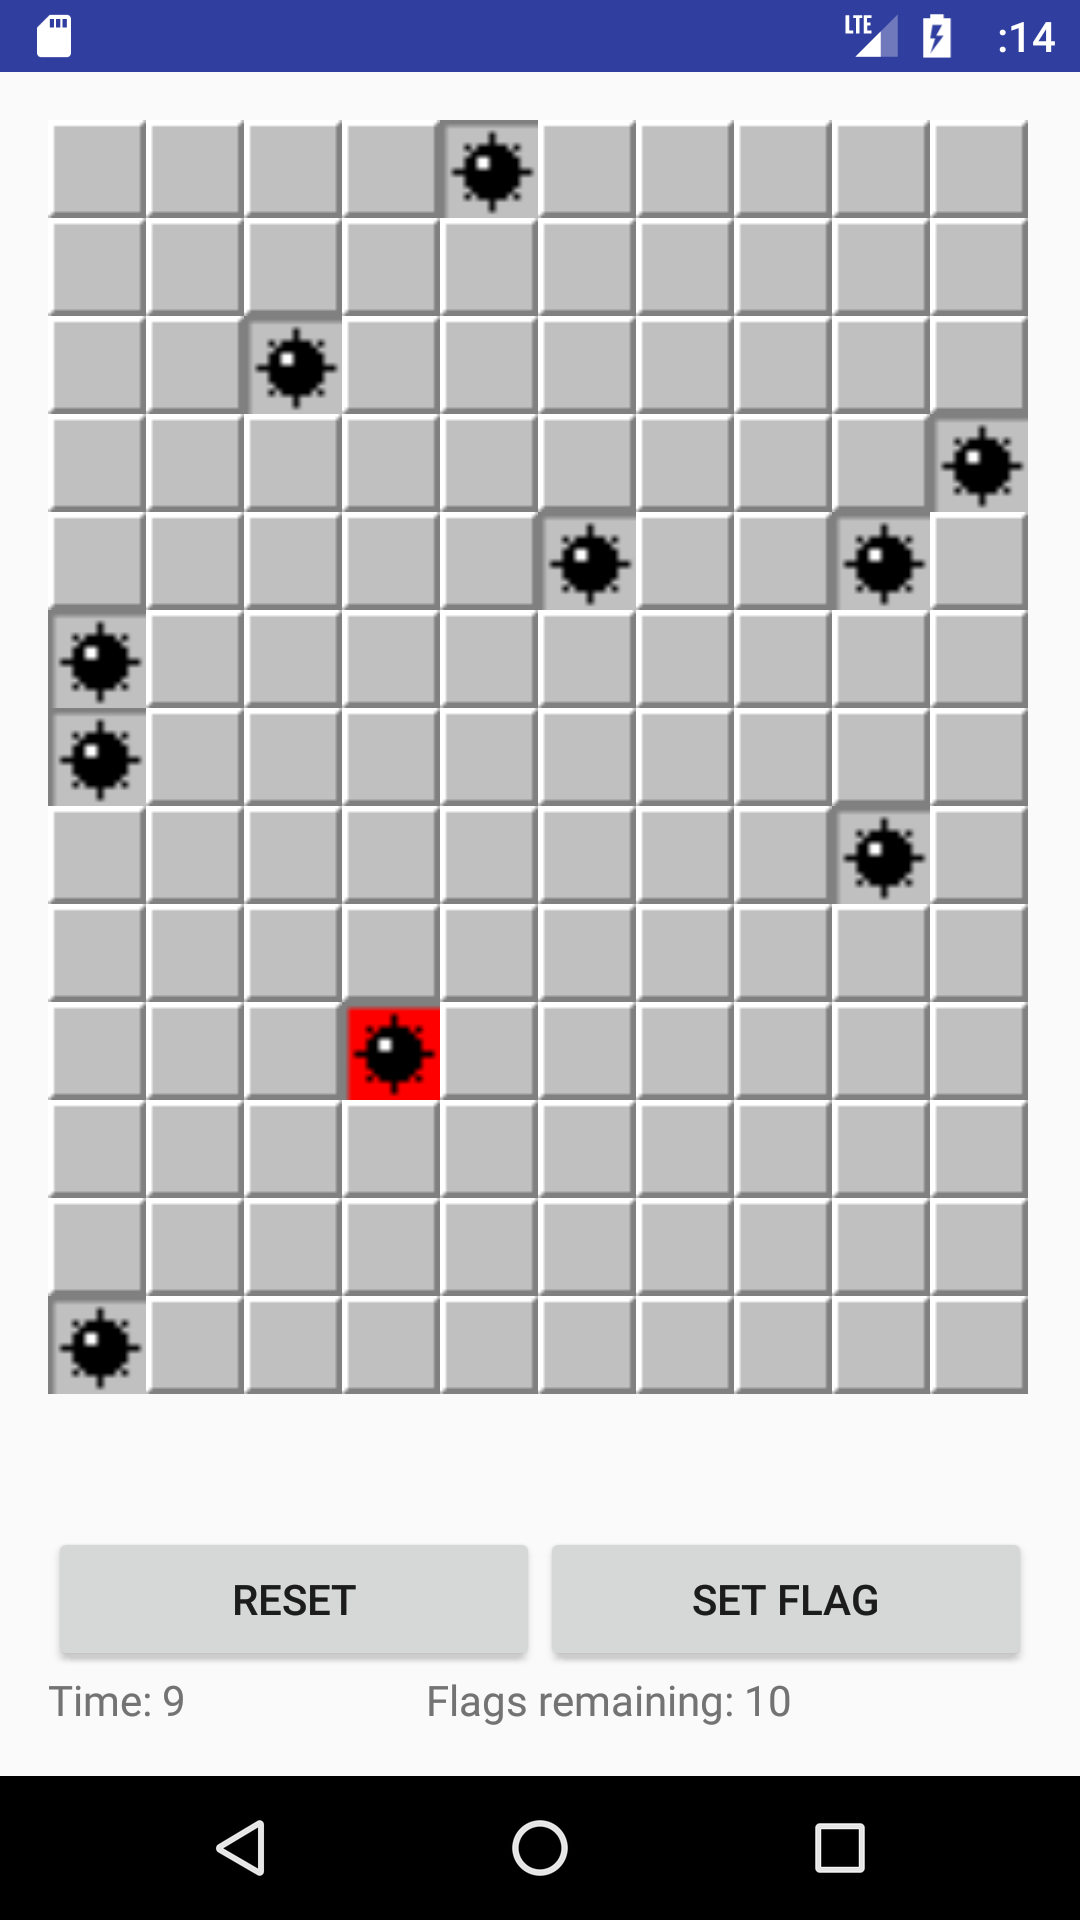
\includegraphics[width=4cm]{img/prohra}\\
	\caption{Bomba vybouchla - konec hry}
	\label{fig:prohra}
	\end{figure}
\par
Pokud uživatel hru dohraje, to znamená odhalí všechna pole neobsahující bombu a označní vlajkama všechna pole, která bombu obsahují, pak je zobrazeno oznámení o~dohrání hry a hra končí. Stejně jako u~prohry může hráč začít hrát novou hru pomocí tlačítka \textit{RESET} nebo hru ukončit. Příklad dohrání hry do úplného konce lze vidět na obrázku \ref{fig:vyhra}.
	\begin{figure}[h!]
	\centering
	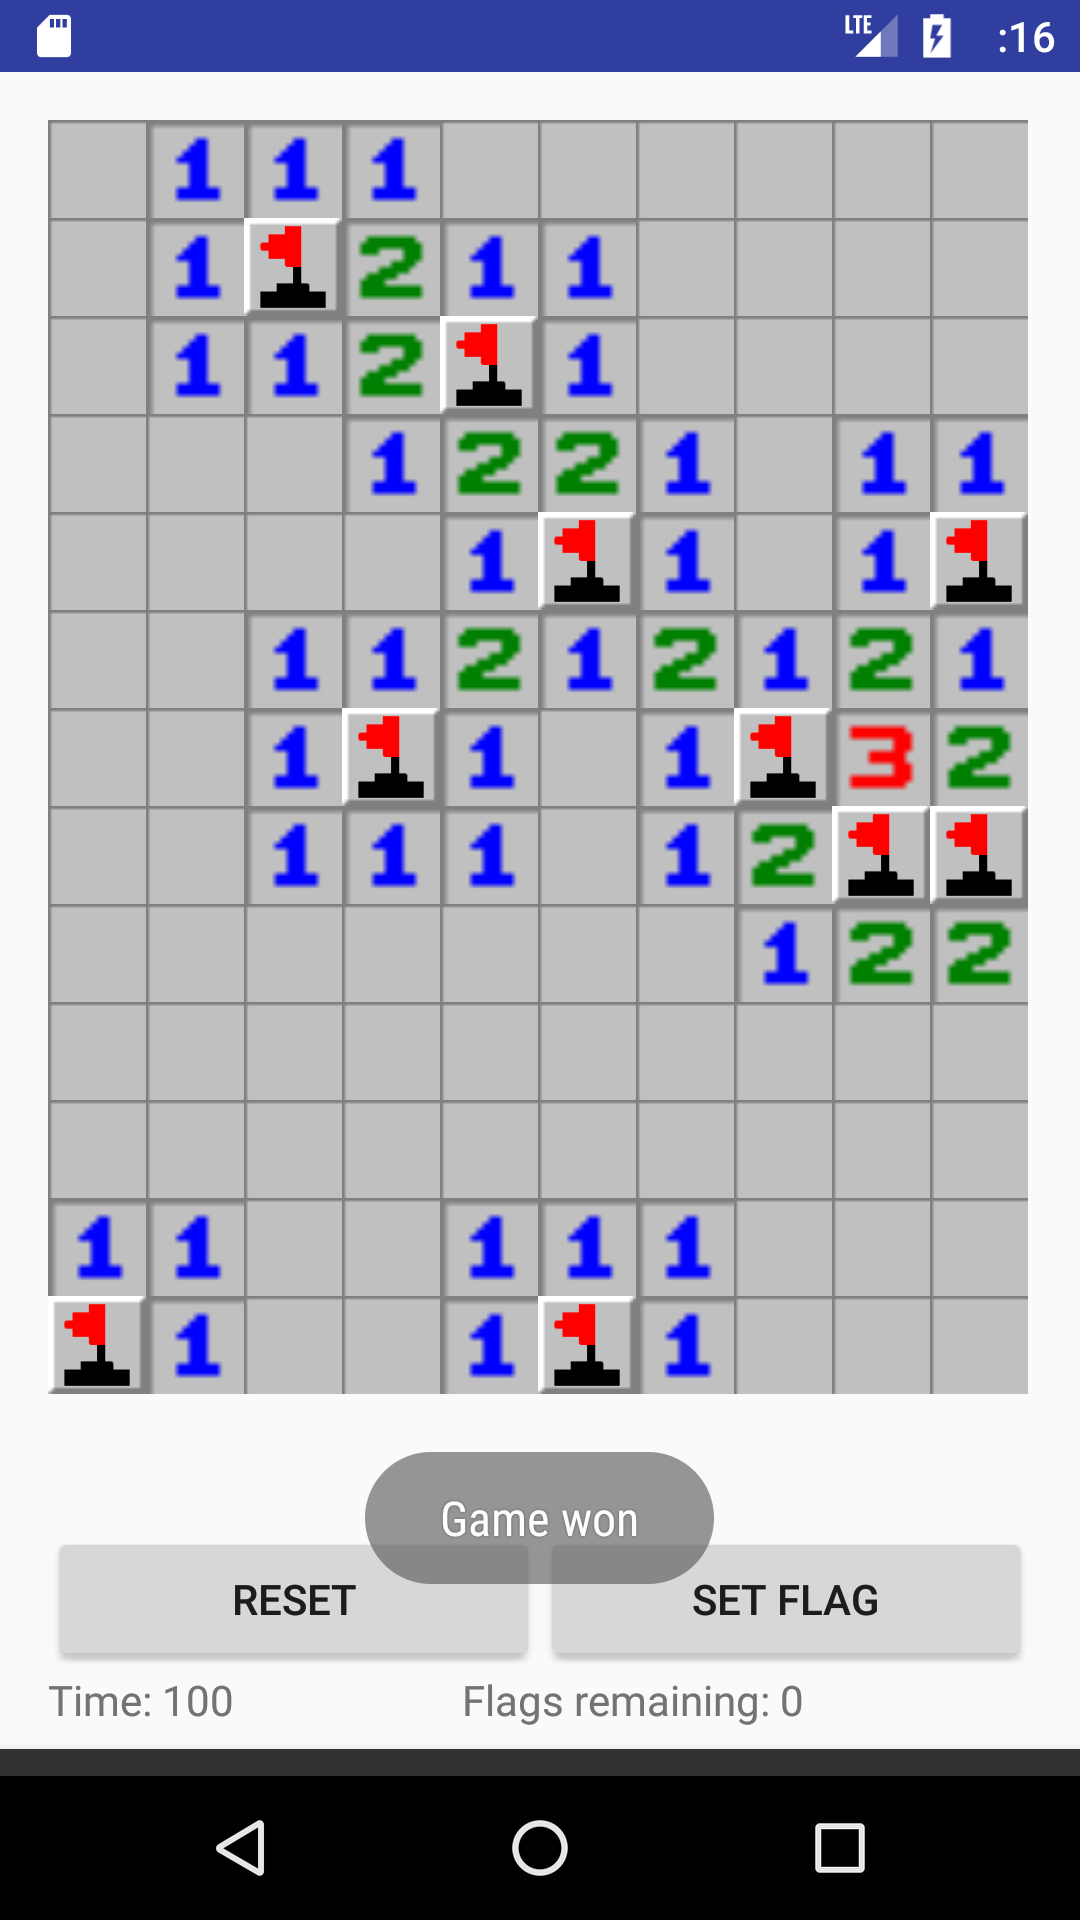
\includegraphics[width=5cm]{img/vyhra}\\
	\caption{Odhalení všech políček a označení všech bomb - výhra}
	\label{fig:vyhra}
	\end{figure}
\newpage


\section{Řešené problémy}
Při vyvíjení aplikace jsem narazil na jeden problém, který spočíval v~nefungování třídy \textbf{Timer} a \textbf{TimerTask}. V~aplikaci funguje časovač, který ukazuje uživatelům počet nahraných sekund v~aktuální hře. Protože třídy Timer a TimerTask se často využívají v~JAVA aplikacích, proto byly zvoleny i pro tuto aplikaci. Při implementování zmíněných tříd ale časovač nefungoval vůbec, důvody nebyly zjištěny. Proto jsem přestoupil na třídu \textbf{CountDownTimer}, která fungovala bez problémů.
\newpage


\section{Testování}
Aplikace byla vyvíjena a testována v~Android Studiu verze 3.3 (od firmy JetBrains) v~jazyce JAVA. Při vývoji bylo využito JRE verze 1.8.0\_152. Jako testovací mobil byl vybrán Nexus 5.2 s~API verzí 24 a operačním systémem Android ve verzi 7.0 (Nougat). 
\par
Aplikace byla testována několika uživateli (převážně studenti ZČU), kteří při hraní hry nenarazili na žádný problém, který by měl fatální dopadek na běh aplikace.
\newpage


\section{Závěr}
Vytvořená mobilní aplikace \textbf{Minesweeper}, neboli hledání min, splňuje základní funkcionalitu stejnojmenné hry. Uživatel je schopný hru bezproblémově dohrát a ukončit ji v~jakémkoliv případě. Ovládání aplikace je velice jednoduché, stačí pouze klikat na políčka v~hracím poli a podle zobrazeného čísla u~některých políček odhadovat, na jakém políčku se můžou nacházet bomby. Bomby jsou rozmístěny náhodně, v~každé hře jsou na jiné pozici. 
\par
Při testování se nevyskytly žádné chyby, které by měli zásadní vliv na funkčnost aplikace. Testovány byly především všechny stavy, které se mohli u~této hry vyskytnout, jako například výhra/prohra, překročení limitu vlajek nebo označení políčka vlajkou i přes to, že už je odhalené.

\end{document}